%\documentclass[aspectratio=169,11pt]{beamer}
\documentclass[11pt]{beamer}

\usetheme{Singapore}
\usepackage[utf8]{inputenc}
%\usepackage{amsmath}
%\usepackage{amsfonts}
%\usepackage{amssymb}
\usepackage{graphicx}
\usepackage{hyperref}
\usepackage{setspace}
%\usepackage{booktabs}
%\usepackage{listings}
%\usepackage{xcolor}
%\usepackage{caption}
%\usepackage{subcaption}

% Set line spacing
\let\oldframetitle\frametitle% Store old \frametitle in \oldframetitle
\renewcommand{\frametitle}[1]{% Redefine \frametitle
  \oldframetitle{#1}\setstretch{1.3}}


% Define the settings for codechunks
%\definecolor{codegreen}{rgb}{0,0.6,0}
%\definecolor{codegray}{rgb}{0.5,0.5,0.5}
%\definecolor{codepurple}{rgb}{0.58,0,0.82}
%\definecolor{backcolour}{rgb}{0.9,0.9,0.9}
%\lstdefinestyle{mystyle}{
%    backgroundcolor=\color{backcolour},   
%    commentstyle=\color{codegreen},
%    keywordstyle=\color{magenta},
%    numberstyle=\tiny\color{codegray},
%    stringstyle=\color{codepurple},
%    basicstyle=\ttfamily\footnotesize,
%    breakatwhitespace=false,         
%    breaklines=true,                 
%    captionpos=b,                    
%    keepspaces=true,                 
%    numbers=left,                    
%    numbersep=5pt,                  
%    showspaces=false,                
%    showstringspaces=false,
%    showtabs=false,                  
%    tabsize=2
%}
%\lstset{style=mystyle}

% Setup the bibliography
%\usepackage[style=authortitle,backend=bibtex,citestyle=verbose]{biblatex}
%\addbibresource{bibliography.bib}
%\setbeamertemplate{bibliography item}[text]
%\setbeamerfont{footnote}{size=\tiny}
%
%% Allow footnotes with no number
%\newcommand\blfootnote[1]{%
%  \begingroup
%  \renewcommand\thefootnote{}\footnote{#1}%
%  \addtocounter{footnote}{-1}%
%  \endgroup
%}

% Allow section title slides
\AtBeginSection[]{
  \begin{frame}
  \vfill
  \centering
  \begin{beamercolorbox}[sep=8pt,center,shadow=true,rounded=true]{title}
    \usebeamerfont{title}\insertsectionhead\par%
  \end{beamercolorbox}
  \vfill
  \end{frame}
}

\author{Stephen Pederson}
\title{DRMCRL}
\subtitle{Group Meeting}
%\setbeamercovered{transparent} 
\setbeamertemplate{navigation symbols}{} 
\logo{
	
\includegraphics[scale=0.25]{../images/UoA_logo_col_vert.png} 
	\hspace{0.84\linewidth}
	
\includegraphics[scale=0.06]{../images/DRMCRL_BANNER_3lines.png} 
} 
\institute{Dame Roma Mitchell Cancer Research Laboratories, \\The University of Adelaide} 
\date{25\textsuperscript{th} August, 2020} 


\begin{document}

\begin{frame}
\titlepage
\end{frame}

\begin{frame}
\tableofcontents
\end{frame}

\section{Introduction}

\begin{frame}{Bioinformatics Hub}

	\begin{itemize}
		\item Co-ordinator Bioinformatics Hub, 2014 - 2020
		\item Currently an ECR: PhD (2008-2018)
		\item Main areas of expertise:
		\begin{itemize}
			\item \texttt{R}, \texttt{bash}, \LaTeX
			\item Transcriptomics and Statistics
		\end{itemize}
	\end{itemize}

\end{frame}

\subsection{Why such a long PhD?}

\begin{frame}{Why such a long PhD?}

	\begin{itemize}
		\item Detect alternate transcript usage using whole-transcript microarrays
		\item Built a Bayesian model which ran a MCMC process (written in C)
		\item Implemented as an R package 
	\end{itemize}

\end{frame}

\begin{frame}{Why such a long PhD?}

	\begin{itemize}
		\item Pre-RStudio, Pre-\texttt{tidyverse}, Pre-\texttt{RMarkdown}, Pre-\texttt{Rcpp}
		\item Model significantly ``under-performed" on real data
		\item Broke the software with no version control strategy 
		\begin{itemize}
			\item MCMC process ran for a week on 4-cores 
			\item Failure was a random failure to complete (probably C memory issues)
			\item Took 6 months to debug
		\end{itemize}
		\item \textit{No bioinformatics community able to help}
	\end{itemize}

\end{frame}

\begin{frame}{Why such a long PhD?}

	\begin{itemize}
		\item Tutored for School of Mathematical Sciences
		\item Picked up large amounts of work as a musician
		\item Landlord died $\implies$ no place to live
		\item Bioinfosummer 2013 (Terry Speed)
	\end{itemize}

\end{frame}

\subsection{The Bioinformatics Hub}

\begin{frame}{Formation of the Bioinformatics Hub}

An application was made to the IDRF

\small

	\begin{enumerate}
		\item Prof David Adelson: Head, School of Biological Sciences; Chair of Bioinformatics
		\item Prof Gary Glonek: Head, School of Mathematical Sciences
		\item Prof Mike Wilkinson: Head, School of Agriculture, Food \& Wine
		\item Prof Julie Owen: Head, School of Paediatrics \& Reproductive Health
	\end{enumerate}
	
Others named with a key interest: \textit{Prof Alan Cooper, Prof Wayne Tilley, Prof Sarah Robertson etc}\\[5mm]

\end{frame}

\begin{frame}{Formation of the Bioinformatics Hub}

	\begin{itemize}
		\item Run bioinformatics training workshops, seminars, journal clubs etc
		\item Manage a hot-desking facility
		\item Provide consultations and advice
		\item Develop formal courses and subjects
		\item Apply for external research funding
		\item Build a \textit{critical mass}
	\end{itemize}
	
	\pause
	Interestingly, this is not a core-facility\\[5mm]

\end{frame}

\begin{frame}{Formation of the Bioinformatics Hub}

	\begin{itemize}
		\item Directors: 
		\begin{itemize}
			\item 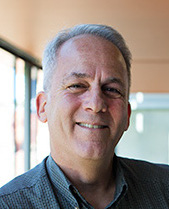
\includegraphics[height=1cm]{figures/dave.jpg} David Adelson (\textit{Biol. Sci.})
			\item 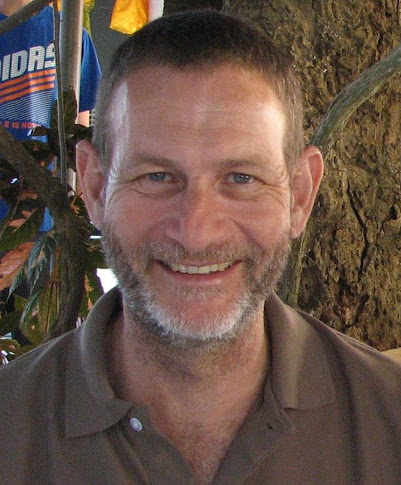
\includegraphics[height=1cm]{figures/gary.jpg} Gary Glonek (\textit{Mathematical Sciences})
		\end{itemize}			
		\item Funded by DVCR to recruit Level B6-C3 Academic for 2014 only
		\item To be administered within School of Biological Sciences (BS)\\[1cm]

	\end{itemize}	
	
\end{frame}

\begin{frame}{Formation of the Bioinformatics Hub}
	
	\begin{itemize}
		\item I commenced in March 2014: 10 month contract at Level A4
	\end{itemize}
	Why?
	\pause
	\begin{itemize}
		\item Not attractive for external recruitment
		\item I was the ``best they could get"\\[2cm]
	\end{itemize}
	
\end{frame}

\begin{frame}{Formation of the Bioinformatics Hub}

In 2015:\\[5mm]

	\begin{itemize}
		\item 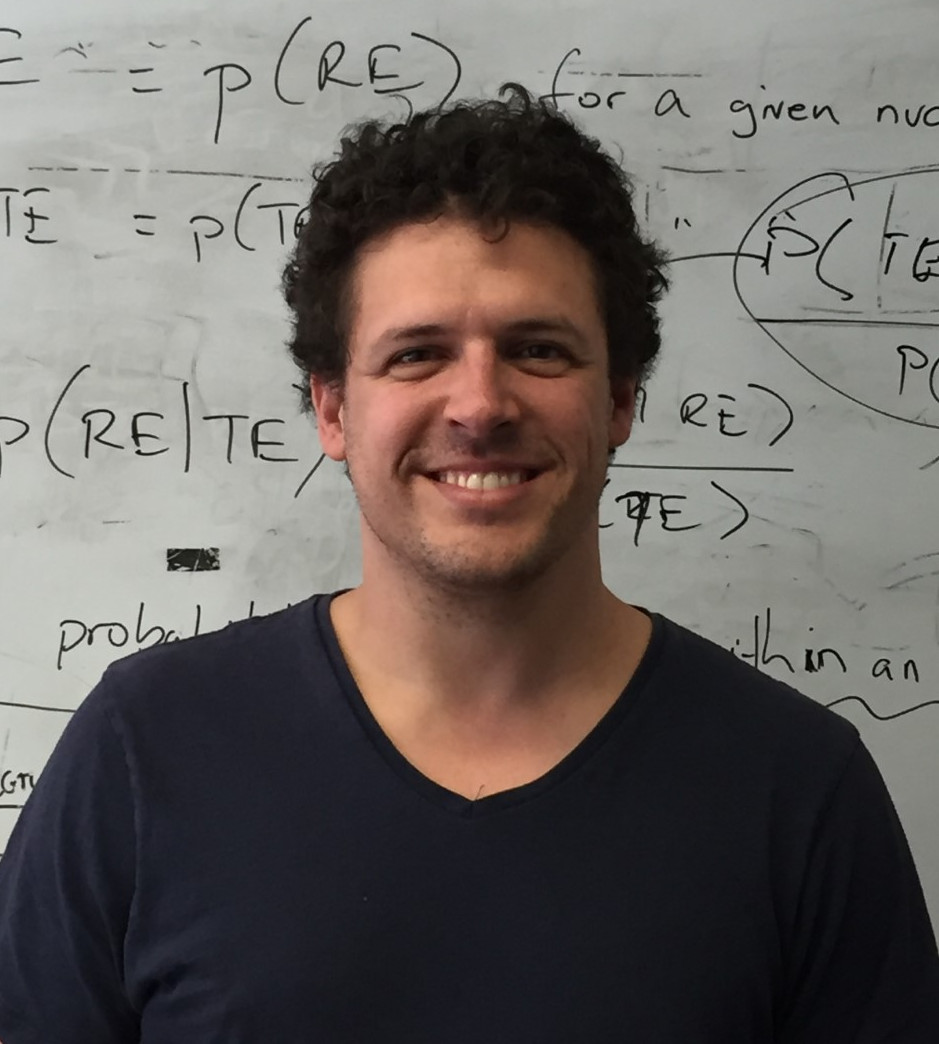
\includegraphics[height=1cm]{figures/Jimmy.jpg} Jimmy Breen appointed to RRI $\implies$ co-located
		\item 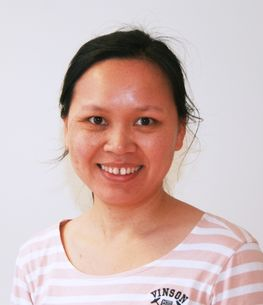
\includegraphics[height=1cm]{figures/hien.jpg} Hien To appointed as second staff member (2015-2018)
		\item 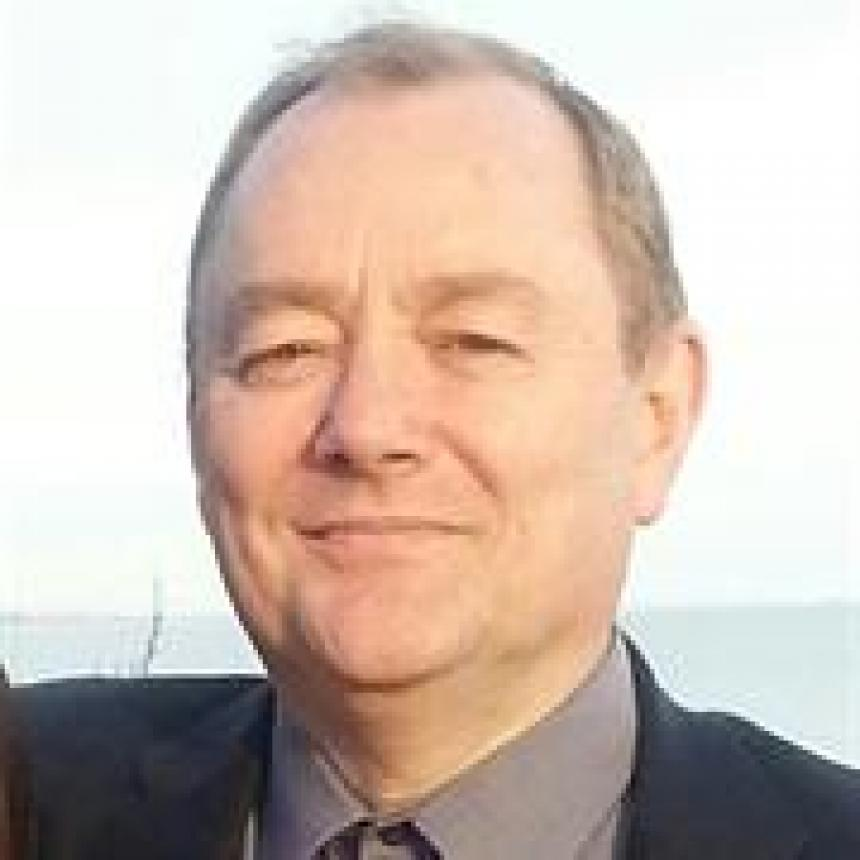
\includegraphics[height=1cm]{figures/rick.jpeg} Rick Tearle appointed to Davies Research Centre (Roseworthy)\\[8mm]
	\end{itemize}		
	
\end{frame}

\begin{frame}{Formation of the Bioinformatics Hub}

Later:\\[5mm]

	\begin{itemize}
		\item 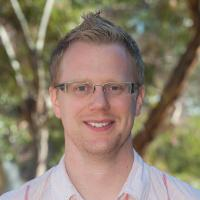
\includegraphics[height=1cm]{figures/Watson-Haigh.jpeg} Nathan Watson-Haigh (2018-2020) 
		\item 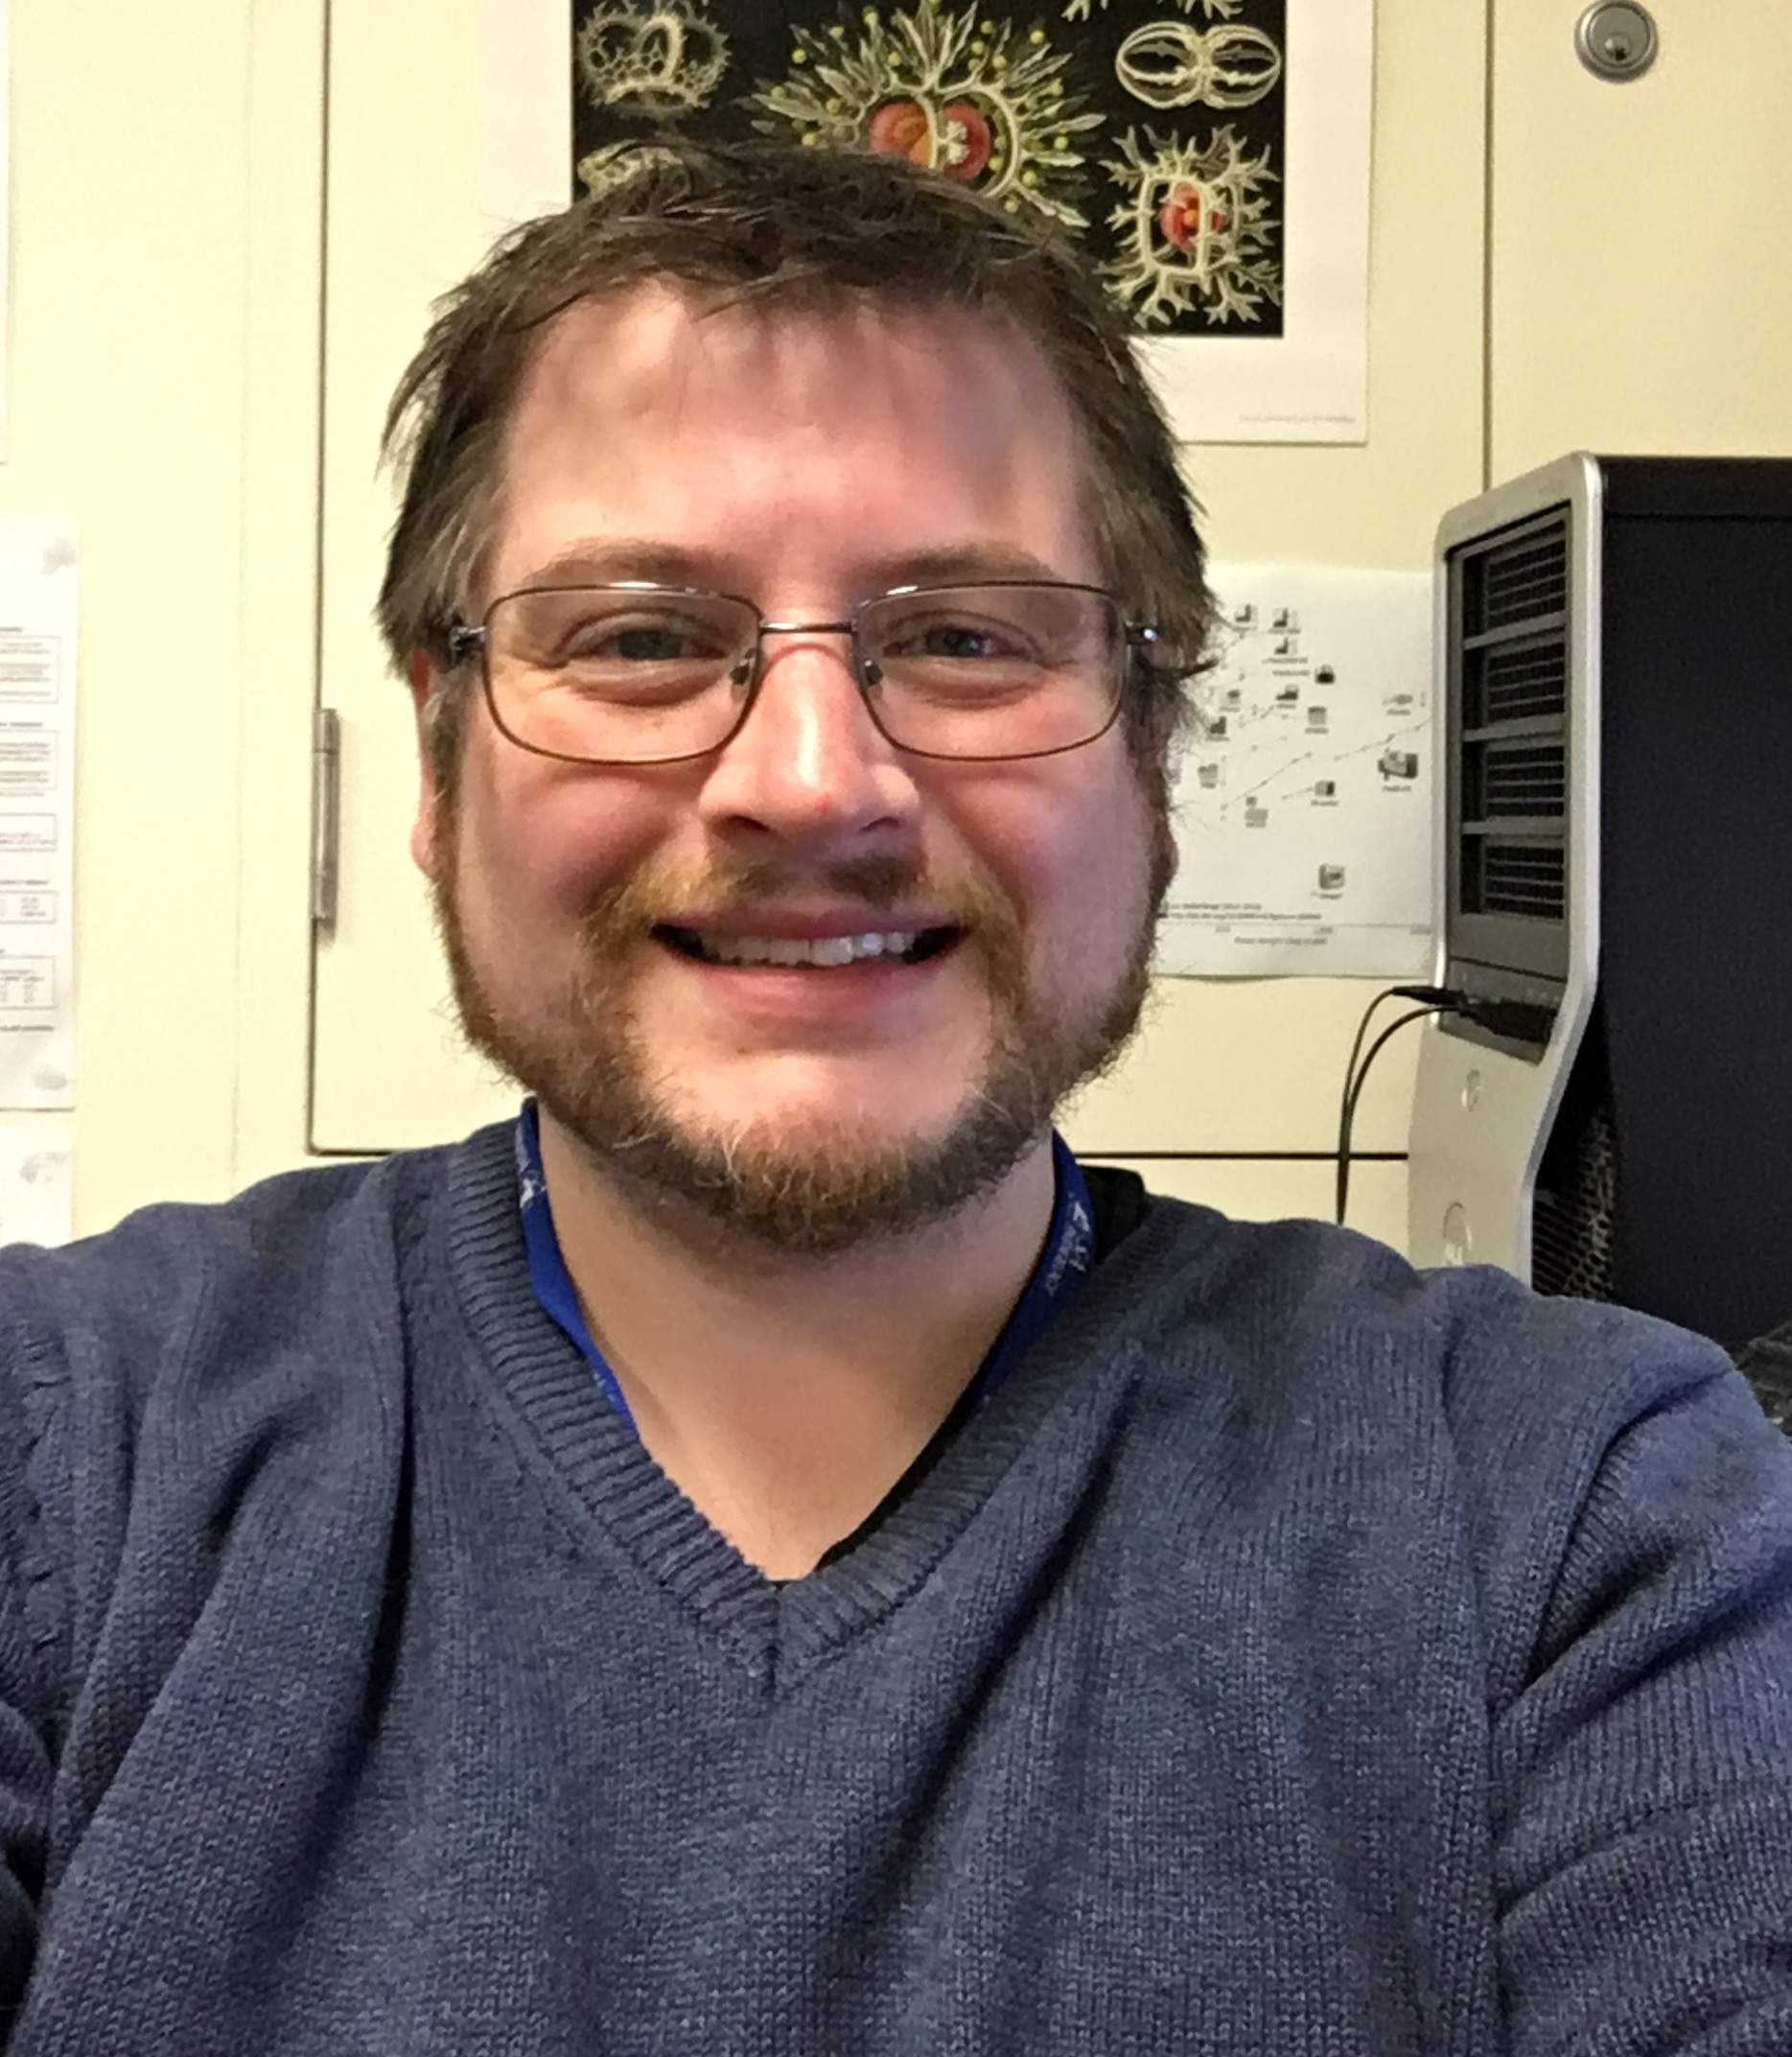
\includegraphics[height=1cm]{figures/Mark.jpg}  Mark Armstrong (2019-2020)
		\item Additional 12 staff members (2015-2020)
	\end{itemize}
	~\\[1cm]
	
\end{frame}


\subsection{Our Track Record}

\begin{frame}{Our Track Record}

Over our existence:

	\begin{itemize}
		\item \$8.5m in grant funding
		\item $>$1400 distinct individuals through workshops
		\item Individual support for $>$360 postgraduate students
		\item Co-authored 84 publications + 2 software packages
		\item Established a Bioinformatics Undergraduate Major
		\item Very strong and supportive bioinformatics community\\[5mm]
	\end{itemize}

\end{frame}

\begin{frame}{Our Track Record}

\small
\center
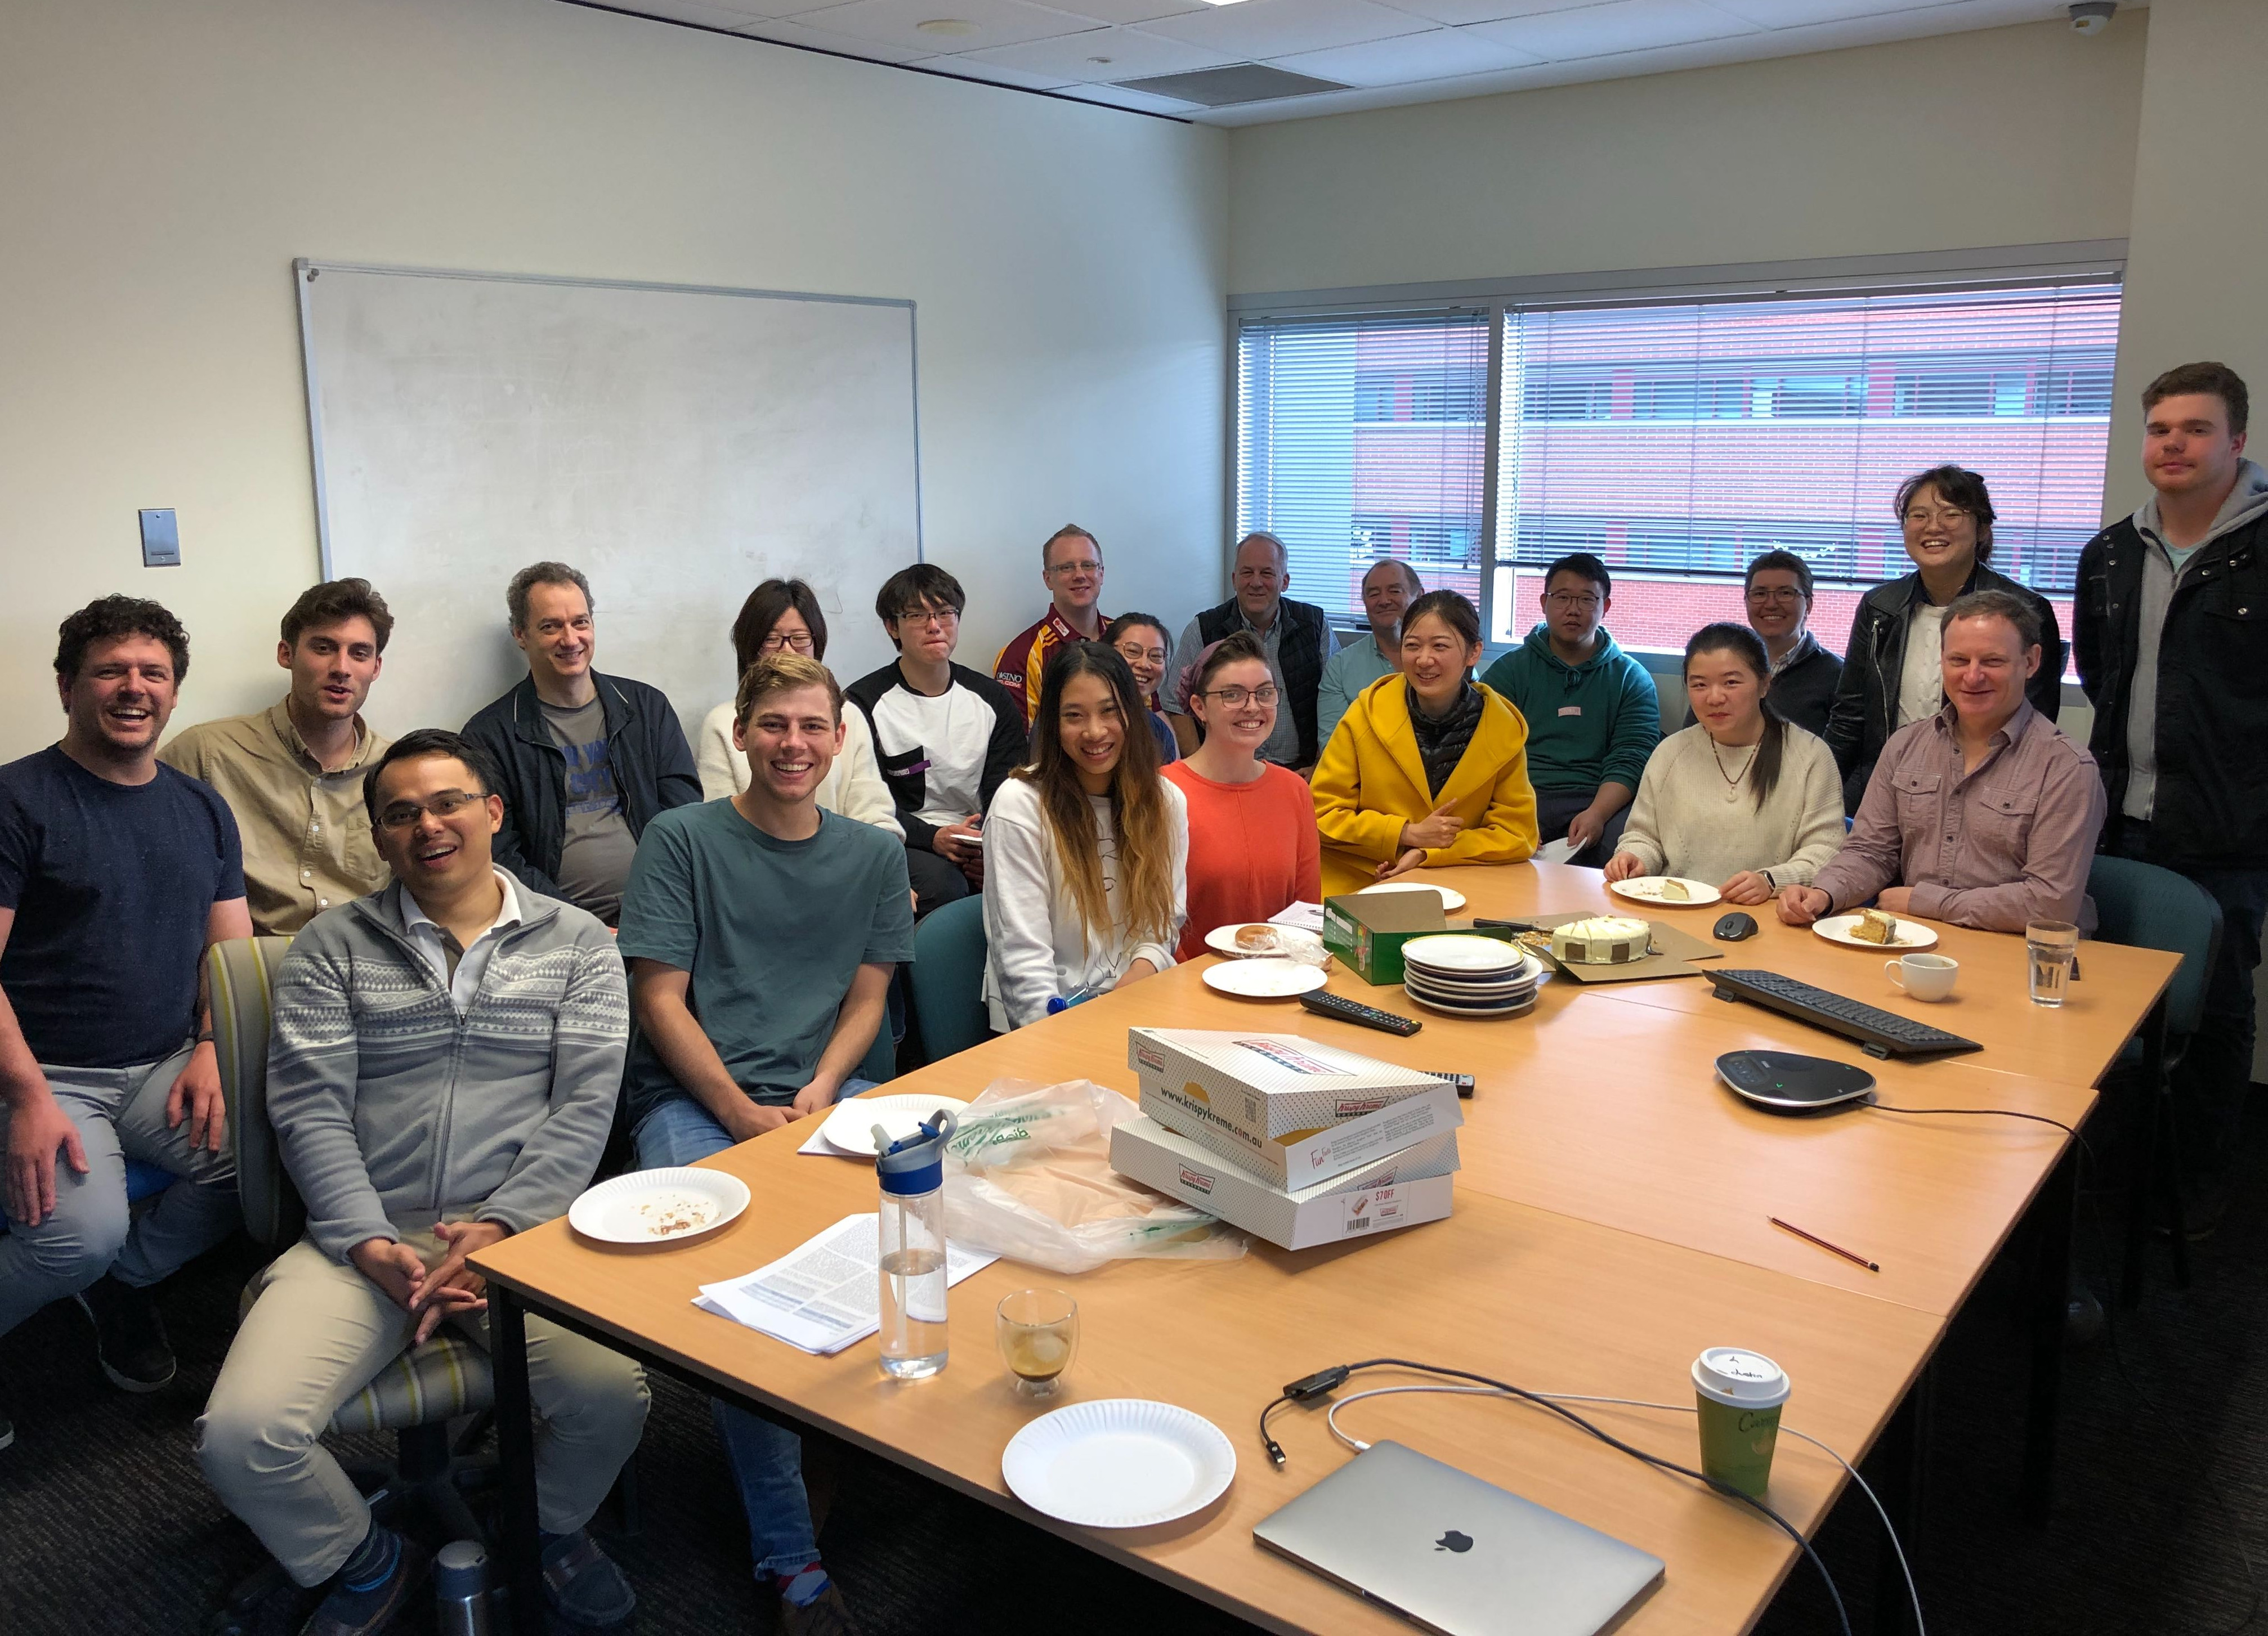
\includegraphics[width=0.75\linewidth]{figures/HubMeetingRoom.jpg}\\
\textit{Journal Club on Steve's Birthday, 2019}\\[1cm]

\end{frame}

\begin{frame}{Publication Highlights}

\center
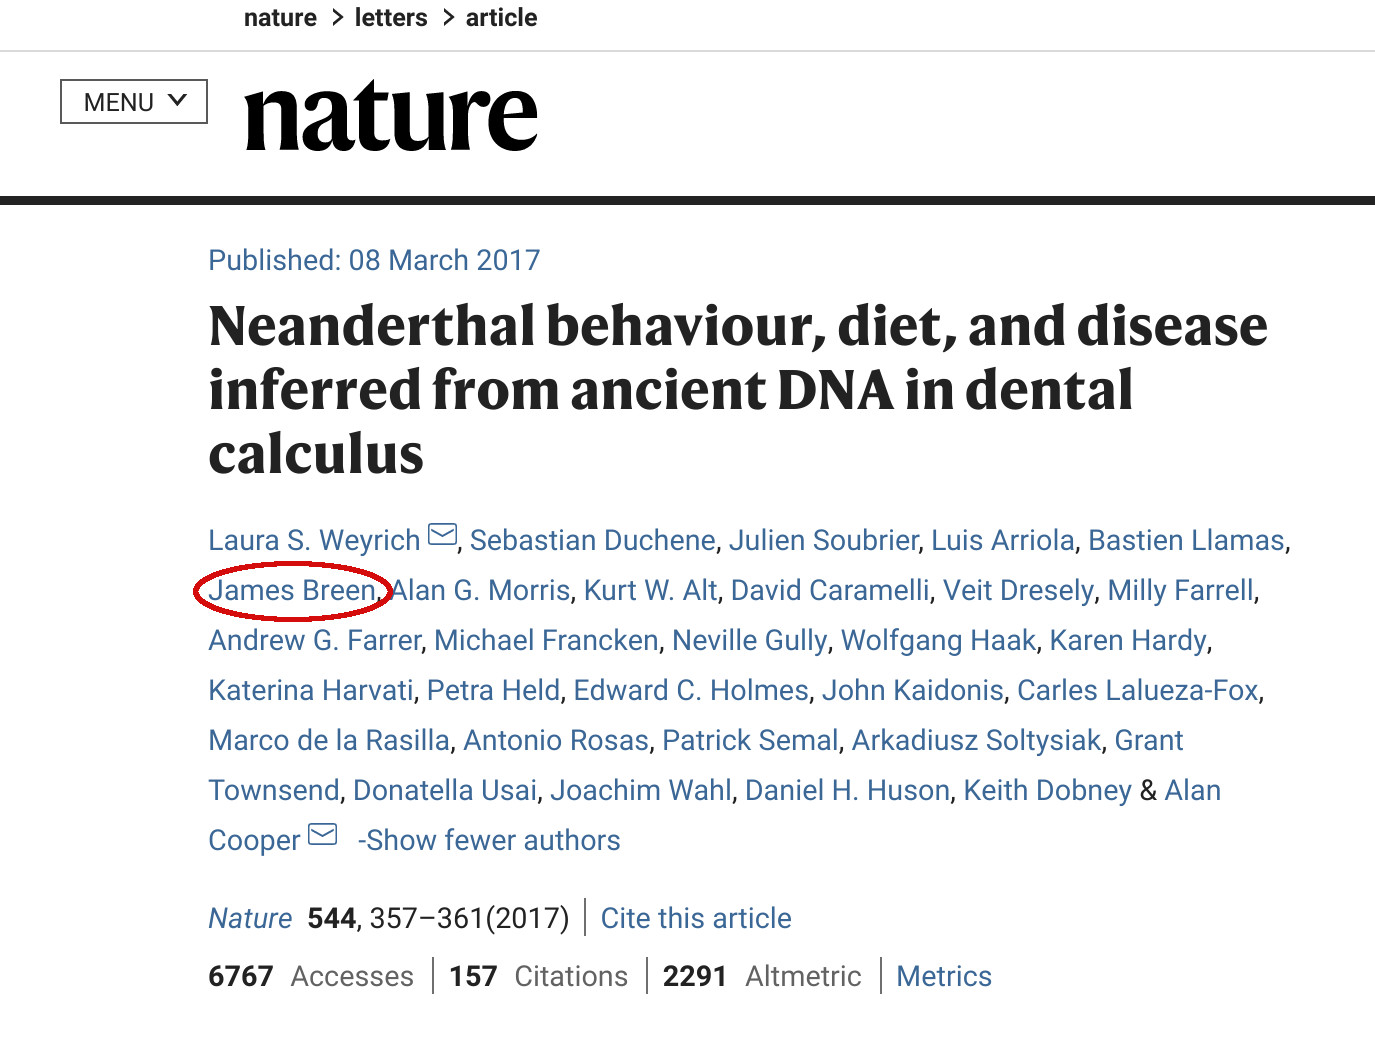
\includegraphics[width=0.7\linewidth]{figures/Nature.jpg} \\[1cm]

\end{frame}

\begin{frame}{Publication Highlights}

\center
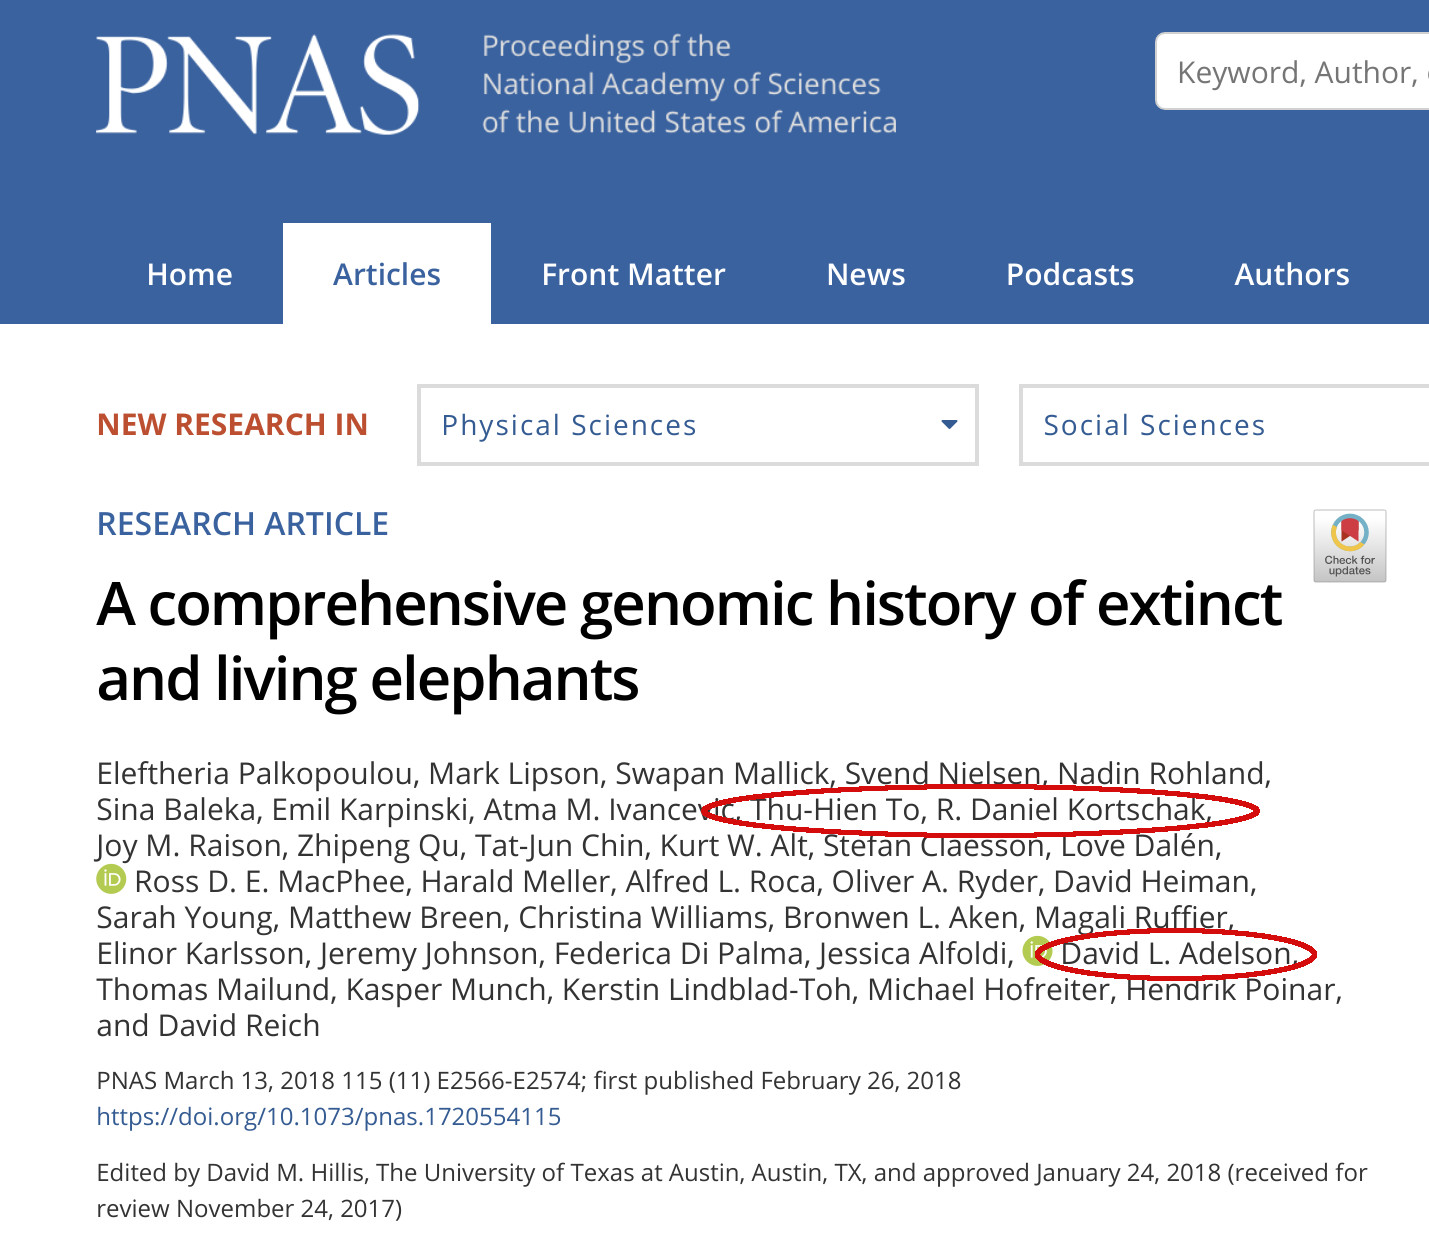
\includegraphics[width=0.7\linewidth]{figures/PNAS.jpg} \\[1cm]

\end{frame}


\begin{frame}{Other Highlights}

	\begin{itemize}
		\item Return on Investment over 6.5 years: \$4.4/dollar
		\item Improved PhD Completion rates (ECMS, Sciences, HMS)
		\begin{itemize}
			\item 66\% with no Hub engagement vs 75\% with ($p = 0.0091$)
		\end{itemize}	
		\item Establishment of UoA as a national player in bioinformatics
		\item Student engagements strongly biased towards women:
		\begin{itemize}
			\item ECMS: 41.7\% Vs 22.0\% (12 students)
			\item HMS: 61.9\% Vs 59.5\% (89 students)
			\item Sciences: 59.2\% Vs 48.3\% (260 students)\\[1cm]
		\end{itemize}
	\end{itemize}

\end{frame}

\begin{frame}{Weaknesses}

	\begin{itemize}
		\item Strategic Vision authored and submitted to Exec Dean of Sciences in 2018
		\item Rejected in it's entirety with no further discussion
		\item Included reimbursement for teaching courses
		\item In 2019 he approved a separate bioinformatics position inside School of BS (still unappointed)\\[1cm]

	\end{itemize}

\end{frame}

\begin{frame}{Weaknesses}

	\begin{itemize}
		\item Income
		\begin{itemize}
			\item Money from grants awarded
			\item Money for course delivery \& student supervision
		\end{itemize}		 
		\item No expectation of reimbursement from DVCR
		\item Short-term contracts made leading grant applications challenging
		\begin{itemize}
			\item I'm too junior
		\end{itemize}
		\item Lack of single ``high-profile" project
		\item How to limit access whilst providing open-access?\\[1cm]
	\end{itemize}

\end{frame}

\begin{frame}{Challenges}

In 6.3 years

	\begin{itemize}
		\item Biological Sciences: 4 Heads of School
		\item Agriculture, Food \& Wine: 4 Heads of School	
	\end{itemize}

\end{frame}

\begin{frame}{SAGC / Our Demise}

	\begin{itemize}
		\item Current DVCR didn't believe he should fund us
		\begin{itemize}
			\item Gave additional money to faculties for these projects
			\item HMS unambiguously supportive whilst Sciences ``receive no benefit at all from the Bioinformatics Hub"
			\item Sciences subsequent internal review found we were beneficial \& vital infrastructure requiring funding
		\end{itemize}
		\item 3 positions provided by UofA as ``in-kind" for SAGC funding 
		\begin{itemize}
			\item 1xDVCR, 1xHMS, 1xSciences
			\item DVCR re-negotiated this down to the HMS position only\\[5mm]
		\end{itemize}
	\end{itemize}

\end{frame}

\begin{frame}{My role}

	\begin{itemize}
		\item I was ready to move on this year
%		\begin{itemize}
%			\item Offered a position at SVI developing scRNA methods
%			\item (The week after state borders closed $\ldots$)
%		\end{itemize}
		\item Being spread across literally everything is exhausting
		\item Being funded on the whims of DVCR, Exec Deans etc is not ideal
		\item Looking to focus more deeply both \textit{biologically} and \textit{bioinformatically}
		\item Take advantage of my ``ECR window"
	\end{itemize}

\end{frame}


\section{Enrichment Analysis}

\section{Incucyte Analysis}


\end{document}